\documentclass[11pt,a4paper,twoside]{book}
\usepackage[utf8]{inputenc}
\usepackage[spanish]{babel}
\usepackage{amsmath}
\usepackage{graphicx}
\usepackage{amsfonts}
\usepackage{amssymb}
\usepackage[left=2cm,right=2cm,top=2cm,bottom=2cm]{geometry}
\usepackage{float}
\author{Víctor de Tejada Molera}
\begin{document}
\chapter{Análisis estadístico}    
    En este capítulo se realiza el análisis estadístico de los resultados que se han obtenido en el test previo y en el segundo test. No se ha incluído el test del primer test puesto que al haberse realizado con señales erróneas, no tiene sentido incluirlos.
    
    En la primera parte del capítulo se comenta brévemente algunos aspectos teóricos de los dos procedimientos que se han aplicado; mientras que en el segundo apartado es donde se refleja el propio análisis.
    \section{Conceptos teóricos}    
        \subsection*{UNE-EN ISO 10399}
            La norma UNE-EN ISO 10399: ``Análisis sensorial. Metodología. Ensayo Duo-Trio.''\cite{ISO10399} es un documento que permite analizar la probabilidad de que eventos perceptuales sean percibidos como iguales o diferentes según el número de respuestas definidas como correctas y/o erróneas al realizar experimentos basados en test duo-trio.
        
            Para ello, en primer lugar se definen diferentes términos que aparecen de forma constante a lo largo de la norma. Para nuestro caso particular, los términos más relevantes son:
        
            \begin{itemize}
                \item alpha-risk o $\alpha$-risk: es la probabilidad para poder afirmar que existe una diferencia perceptual cuando en realidad no existe.
                \item beta-risk o $\beta$-risk: es la probabilidad para poder afirmar que no existe una diferencia perceptual cuando en realidad sí existe.
                \item diferencia perceptual: situación en la que dos o maś muestras pueden ser distinguidas por sus propiedades sensitivas (a través del oído, tacto, gusto, vista, etc.)
                \item similaridad perceptual: situación en la que las diferencias entre muestras son tan pequeñas que no pueden distinguirse entre sí de forma sensitiva.
            \end{itemize}
            Para el cálculo de las probabilidades $\alpha$-risk y $\beta$-risk, la norma proporciona dos sendas tablas que se encuentran en el Anexo A de dicha norma (las tablas A.1 y A.2 respectivamente). También se proporciona la ecuación \ref{eq:alpha} donde se puede calcular el mínimo de respuestas ``correctas'' para que se obtenga un determinado valor de $\alpha$-risk.
            
            \begin{equation}
                x=(n/2)+z*\sqrt{n/4}
                \label{eq:alpha}
            \end{equation}
            
            Donde:
            \begin{itemize}
                \item x: número de respuestas correctas mínimas necesarias para que se obtenga un determinado $\alpha$-risk.
                \item n: número de respuestas totales.
                \item z: variable que toma un valor en función de $\alpha$-risk:
                \begin{itemize}
                    \item 0.84 para $\alpha=0.20$.
                    \item 1.28 para $\alpha=0.10$.
                    \item 1.64 para $\alpha=0.05$.
                    \item 2.33 para $\alpha=0.01$.
                    \item 3.09 para $\alpha=0.001$.
                    
                \end{itemize}
            \end{itemize}
        \subsection*{Modelos Thursthonianos}
            Los modelos Thursthonianos son modelos estadísticos en el que se utilizan variables de distribuciones normales y que se utilizan en gran medida en estudios de discriminación sensorial. 
            
            En el caso concreto de la psicoacústica, se utiliza generalmente para obtener un valor ``$d'$'' que da información ordenada y cuantitativa sobre una determinada percepción subjetiva. Además de este valor, se calcula a su vez la desviación estandar ``$\sigma$''. Con estos dos valores, se puede aproximar un conjunto de distribuciones como una sucesión de distribuciones gaussianas en las que en función del valor ``$d'$''y ``$\sigma$'' están más o menos superpuestas. Esta superposición da información sobre la probabilidad de que ambos estímulos puedan ser distinguibles o no entre sí y cuánto. Esto se observa más fácilmente en la figura \ref{fig:modelost} obtenida en \cite{PsychophysicsB} 
            
            \begin{figure}
                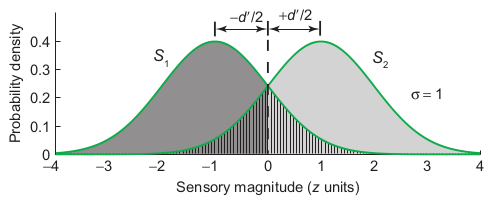
\includegraphics[scale=0.7]{../imagenes/modelosthurst.png}
			    \centering
			    \caption{Ejemplo de cálculo de d' utilizando modelos thursthonianos. Fte: \cite{PsychophysicsB} }
			    \label{fig:modelost}
            \end{figure}
            
            Además de lo ya expuesto, este tipo de análisis es especialmente interesante porque nos permite ordenar los valores obtenidos para $d'$ de forma que las diferencias entre ellos nos da información cuantitativa sobre cómo de diferentes o de similares son cada una de las distribuciones. Con la facilidad añadida que tiene este sistema para representar gráficamente mediante las técnicas habituales como diagramas de barras, entre otros.
            
    \section{Análisis de los resultados}
        En este apartado, se muestran los diferentes análisis que se han realizado para los diferentes test; así como los procedimientos utilizados para su obtención.
        
        \subsection{Análisis del test previo}
            Para este test sólo se pretende comprobar si las personas eran capaces de distinguir entre audios en posiciones muy diferentes. Por este motivo, se decidió realizar un análisis más sencillo que en el caso del test final. Más concretamente, se optó por utilizar la tabla A1 del anexo A de la norma UNE-EN ISO 10399, así como la ecuación \ref{eq:alpha}.
            
            Aplicando dichos recursos se obtienen las tablas \ref{tablaResultadosDuda} y \ref{tablaResultadosSinDuda} en la que se incluyen todas respuestas y únicamente las que se marcaron como ``seguras'' por parte de los participantes respectivamente:
            
            \begin{table}
			\begin{center}
			\begin{scriptsize}
			\begin{tabular}{| c | c | c | c || c |}
			    \hline
				\textbf{Separación butacas}&\textbf{Respuestas}&\textbf{Total iguales}&\textbf{Total diferentes}&\textbf{$\alpha$-risk}\\ \hline
                Horizontal&27&9&18&0.1\\ \hline
                Vertical&10&1&9&0.01\\ \hline
                Horizontal y vertical&23
                &5&18&0.01\\ \hline
                Misma posición&10&9&1&NO\\ \hline
			\end{tabular}
			\caption{Resultados del test previo.}
			\label{tablaResultadosDuda}
			\end{scriptsize}
			\end{center}	
		\end{table}	
		
		\begin{table}
			\begin{center}
			\begin{scriptsize}
			\begin{tabular}{| c | c | c | c || c |}
			    \hline
				\textbf{Separación butacas}&\textbf{Respuestas}&\textbf{Total iguales}&\textbf{Total diferentes}&\textbf{$\alpha$-risk}\\ \hline
                Horizontal&23&7&16&0.05\\ \hline
                Vertical&9&1&8&0.05\\ \hline
                Horizontal y vertical&20&4&16&0.01\\ \hline
                Misma posición&9&8&1&NO\\ \hline
			\end{tabular}
			\caption{Resultados del test previo.}
			\label{tablaResultadosSinDuda}
			\end{scriptsize}
			\end{center}	
		\end{table}
		
		Como se puede observar de las tablas ya mencionadas, existen diferencias estadísticamente significativas cuando se separan los puntos de escucha. Dicho efecto se sigue manteniendo cuando se suprimen las respuestas marcadas como ``No seguras''. Por este motivo, se considera probada nuestra primera hipótesis y se decidió continuar con el estudio.
		
		Los valores obtenidos para $\alpha$-risk no son realmente importantes, puesto que el número de datos es relativamente pequeño y la repetición de dicho experimentos podría producir que dichos valores fluctuaran. No obstante, para este caso resultaba válido con obtener valores superiores y/o iguales a 0.1, que es lo que se ha obtenido.
		
		También se obtienen los resultados esperados para los casos en que ambos audios se encuentran en la misma posición, donde la amplia mayoría de las personas participantes no percibían los estímulos como diferentes.
		
    \subsection{Análisis del test final}
    
		
            
            
            
\bibliography{biblio.bib}
\bibliographystyle{ieeetr}    
\end{document}